\subsection{FACT Data Analysis}
The first use-case we focus on is data pre-processing in the
domain of scientific data obtained from a radio telescope. The
FACT project maintains a telescope for recording cosmic showers
in a fine grained resolution. The telescope consists of a mirror
area which has a 1440-pixel camera mounted on top. This camera
is recording electric energy-impulses which in turn is measured
by sampling each pixel at a rate of 2 GHz.

Based on trigger-signals, small sequences (a few
nanoseconds) of these energy-impulses are recorded and stored into 
files. Each sequence is regarded as a single {\em event}. 
The electronics of the telescope are capable of recording about
60 events per second, resulting in a data volume of up to 10 GB
of raw data that is recorded over a 5 minute runtime. The captured
data of those 5-minute runs is stored in files.
% using the FITS format.

%\bigskip

The long-term objective of analyzing the FACT data comprises several tasks:
\begin{enumerate}
  \item Identify events that represent showers.
  \item Classify these events as Gamma or Hadron showers.
  \item Use the Gamma events for further analysis with regard to physics stuff.
\end{enumerate}

Besides the pure analysis the data has to be pre-processed in order
to filter out noisy events, calibrate the data according to the state
of the telescope electronic (e.g. stratify voltages over all camera pixels).

%As can be seen in Figure \ref{fig:eventStream}, the basic view of the 
%FACT data is that of a continuous stream of events. The plugin provides
%a FACT-stream operator that allows to open a (compressed) FACT file in FITS format
%and also implements the DRS calibration used to calibrate the RAW
%data. The outcome is a stream of calibrated event objects.

%A {\em DataStreamProcessing} operator can then be attached to that
%stream to iteratively process the stream event-by-event. That way,
%only a single event is read into main memory at a time.

%\subsubsection{Processing Data of the FACT Telescope}
%
%This raw data needs an additional calibration before any furthr analysis
%can be applied. An abstract outline of the FACT analysis is shown in
%Figure \ref{fig:eventStream}.

\begin{figure}[h!]
\begin{center}
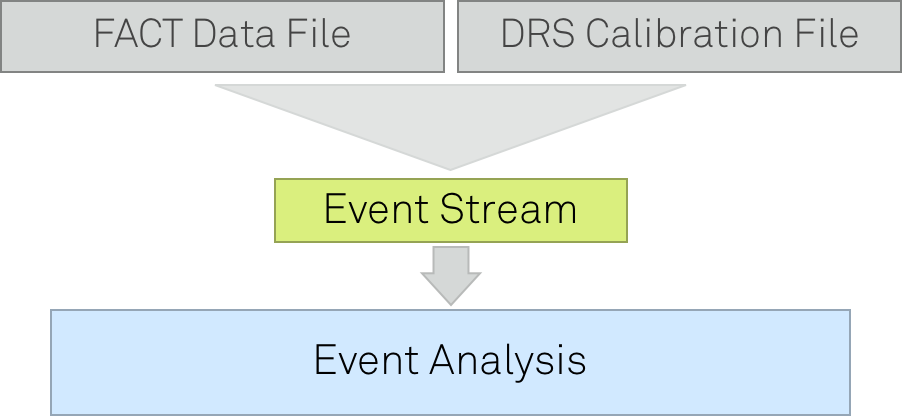
\includegraphics[scale=0.2]{fact-event-stream}
\end{center}
\caption{\label{fig:eventStream}Stream-lined processing of events.}
\end{figure}





\subsubsection{Reading FACT Data}
The {\em fact-tools} library is an extension of the \streams framework that
adds domain specific implementations such as stream-sources and specific 
processors to process FACT data stored in FITS files. These processors provide
the code for calibrating the data according to previously observed parameters,
allow for camera image analysis (image cleaning) or for extracting features
for subsequent analysis.

The XML snippet in Figure \ref{fig:readFACTxml} defines a simple process to
read raw data from a FITS file and apply a calibration step to transform that
data into correct values based upon previously recorded calibration parameters.

\begin{figure}[h!]
\begin{lstlisting}{language=XML}
    <container>
        <stream id="factData" url="file:/data/2011-09-13-004.fits.gz"
             class="fact.io.FACTEventStream" />
        <process input="factData">
             <fact.io.DrsCalibration file="/data/2011-09-13-001.fits.drs.gz" />
             <!--  add further processors here  -->
        </process>
    </container>
\end{lstlisting}
\caption{\label{fig:readFACTxml}Basic process definition for reading raw FACT data
and calibrating that data.}
\end{figure}

Each single event that is read from the event stream, contains the
full raw, calibrated measurements of the telescope. 
%As with all other
%data stream implementations, the {\em FactEventStream} emits a sequence
%of {\em data items}, each of which contains the data of a single FACT
%event.
The attributes of the data items reflect the image data, event
meta information and all other data that has been recorded during the
observation. Table \ref{tab:factEventKeys} lists all the attributes of
an event that are currently provided by the {\ttfamily FACTEventStream}
class.
\begin{table}[h!]
\renewcommand{\arraystretch}{1.25}
{\footnotesize
  \begin{center}
    \begin{tabular}{l|l} \hline
      \textsf{\textbf{Name (key)}} & \textsf{\textbf{Description}} \\ \hline \hline
      {\ttfamily EventNum} & The event number in the stream \\ \hline
      {\ttfamily TriggerNum} & The trigger number in the stream \\ \hline
      {\ttfamily TriggerType} & The trigger type that caused recording of the event \\ \hline
      {\ttfamily NumBoards} & \\ \hline
      {\ttfamily Errors} & \\ \hline
      {\ttfamily SoftTrig} & \\ \hline
      {\ttfamily UnixTimeUTC} & \\ \hline
      {\ttfamily BoardTime} & \\ \hline
      {\ttfamily StartCellData} & \\ \hline
      {\ttfamily StartCellTimeMarker} & \\ \hline
      {\ttfamily Data} & The raw data array ($1440\cdot 300 = 432000$ float values) \\ \hline
      {\ttfamily TimeMarker} & \\ \hline
      {\ttfamily @id} & A simple identifier providing date, run and event IDs \\ \hline
      {\ttfamily @source} & The file or URL the event has been read from \\ \hline
    \end{tabular}
  \end{center}}
  \caption{\label{tab:factEventKeys} The elements available for each event.}
\end{table}

The {\ttfamily @id} and {\ttfamily @source} attributes provide meta-information that is added by
the FACT-stream implementation itself, all the other attributes are provided within
the FITS data files. The {\ttfamily @id} attribute's value is created
from the {\ttfamily EventNum} and date, e.g. {\ttfamily
  2011/11/27/42/8}, denoting the event 8 in run 42 on the 27th of
November 2011.


\subsubsection{Processors for FACT Data}
Any of the existing core processors of the \streams library can directly be applied
to data items of the FACT event stream. This already allows for general applications
such as adding additional data (e.g. whether data from a database).

The {\em fact-tools} library provides several domain specific processors that focus
on the handling of FACT events. The {\ttfamily DrsCalibration} processor for calibrating
the raw data has already been mentioned above.

Other processors included are more specifically addressing the image-analysis task:
\begin{itemize}
  \item {\ttfamily fact.data.CutSlices} \\
  Which can be used to select a subset of the raw data array for only a excerpt of
  the region-of-interest\footnote{The {\em region of interest} is the length of the
  recorded time for each event, usually 300 nanoseconds, at most 1024 nanoseconds} (ROI).

  \item {\ttfamily fact.data.SliceNormalization} \\
  As there is a single-valued series of floats provided for each pixel, this processor
  allows for normalizing the values for these series to $[0,1]$.

  \item {\ttfamily fact.data.MaxAmplitude} \\
  This processor extracts a float-array of length 1440, which contains the maximum
  amplitude for each pixel.

  \item {\ttfamily fact.image.DetectCorePixel} \\
  This class implements a heuristic strategy to select the possible core-pixels of
  a shower, that may be contained within the event.
\end{itemize}


\subsection*{Installing the FACT-Plugin}
The FACT-Plugin is an extension for RapidMiner. The RapidMiner
open-source software is written in Java and is available for multiple
environments (Windows, Unix). It can be downloaded from
\url{http://rapid-i.com}.

The FACT-Plugin is a simple Java archive ({\em jar}-file) that can be
found at
\begin{displaymath}
 \mbox{\url{http://sfb876.tu-dortmund.de/FACT/}}
\end{displaymath}
To install the plugin simply copy the latest {\ttfamily FACT-Plugin.jar}
to your RapidMiner {\ttfamily lib/plugins} directory. After restarting
RapidMiner, the plugin will be loaded and all of its additional operators
will show up in the operators list.



